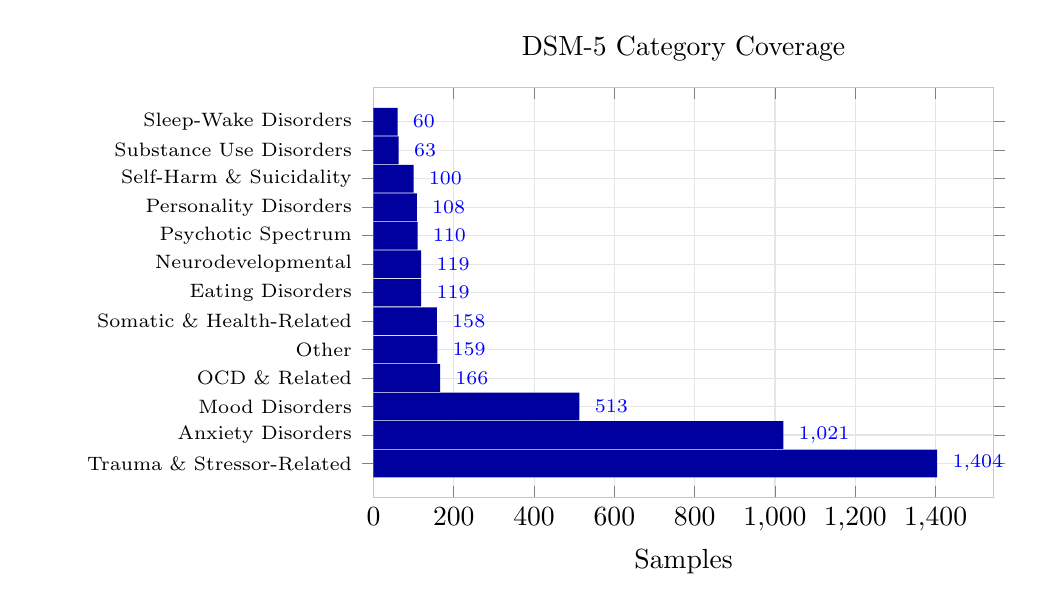
\begin{tikzpicture}
\begin{axis}[
  width=0.78\textwidth,
  height=0.56\textwidth,
  xbar,
  xmin=0,
  ytick=data,
  yticklabels={{Trauma \& Stressor-Related},{Anxiety Disorders},{Mood Disorders},{OCD \& Related},{Other},{Somatic \& Health-Related},{Eating Disorders},{Neurodevelopmental},{Psychotic Spectrum},{Personality Disorders},{Self-Harm \& Suicidality},{Substance Use Disorders},{Sleep-Wake Disorders}},
  yticklabel style={font=\scriptsize, text width=4.0cm, align=right},
  xlabel={Samples},
  title={DSM-5 Category Coverage},
  nodes near coords,
  every node near coord/.append style={font=\scriptsize, xshift=2pt},
  grid=major,
  grid style={draw=gray!20},
  axis line style={draw=gray!45},
]
\addplot+[draw=none, fill=blue!62!black] coordinates {(1404,0) (1021,1) (513,2) (166,3) (159,4) (158,5) (119,6) (119,7) (110,8) (108,9) (100,10) (63,11) (60,12)};
\end{axis}
\end{tikzpicture}
